\documentclass[conference]{IEEEtran}
\IEEEoverridecommandlockouts
\usepackage{fontspec}
\usepackage{amsmath}
\usepackage{unicode-math}
\setmainfont{STIX Two Text}
\setmathfont{STIX Two Math}
\usepackage{cite}
\usepackage{algorithmic}
\usepackage{graphicx}
\usepackage{textcomp}
\usepackage{xcolor}
\usepackage{booktabs,array}
\usepackage{float}
\graphicspath{{figures/}}
\def\BibTeX{{\rm B\kern-.05em{\sc i\kern-.025em b}\kern-.08em
    T\kern-.1667em\lower.7ex\hbox{E}\kern-.125emX}}


% Number of participants in the current analyses (update when more subjects are added)
\newcommand{\Nsub}{8}

\begin{document}

\title{Category and Load Effects in HCP Working Memory and Language Task-fMRI: \\ A Pattern-Based Model of Task Demands}

\author{\IEEEauthorblockN{1\textsuperscript{st} Sai Veeksha Tavva}
\IEEEauthorblockA{\textit{IIT Hyderabad} \\
Roll No.\ 2024113021}
\and
\IEEEauthorblockN{2\textsuperscript{nd} Sahishnu Pawan Kumar}
\IEEEauthorblockA{\textit{IIIT Hyderabad} \\
Roll No.\ 2024113016}
}

\maketitle

\begin{abstract}
Working-memory tasks impose a domain-general demand (memory load) and a content-specific demand (what is held). We model how multivoxel task-fMRI patterns from the Human Connectome Project organise these two demands, using a two-stage encoding and representational model, own implementations of the GLM, cross-validated RSA and decoding, a resting-state null, and a visual-to-auditory demand-transfer test. Results and discussion are to be added.
\end{abstract}

\begin{IEEEkeywords}
working memory, task fMRI, representational similarity analysis, decoding, representational geometry
\end{IEEEkeywords}

\section{Aim of the Modelling Exercise}
\label{sec:aim}

The aim is to build and test a quantitative, pattern-based model of how the brain's response to a working-memory (WM) task is organised by two kinds of demand: a domain-general demand set by memory \emph{load}, and a content-specific demand set by the \emph{category} of what is held (faces, places, tools, body parts). Using Human Connectome Project (HCP) task-fMRI, we ask which regions carry which kind of information and whether the code for one survives a change in the other.

\textbf{Research question.} Do multivoxel activity patterns differ between stimulus categories, and does this category information persist when load rises from 0-back to 2-back? Is the load-related signal shared between a visual task (N-back) and an auditory task (Language: Math versus Story)?

We test four hypotheses, each with a pre-specified analysis and null:
\begin{itemize}
\item \textbf{H1 (category patterns).} Each category evokes a distinct, reproducible pattern in occipito-temporal (OT) cortex, distributed rather than carried only by the most selective voxels.
\item \textbf{H2 (dissociation, invariance).} Load is carried mainly by dorsal frontoparietal and cingulate regions and category by OT cortex; the category code is preserved across loads, so a category decoder transfers across load.
\item \textbf{H3 (control).} Both effects exceed a null built from resting-state fMRI (rfMRI) analysed with the same pipeline.
\item \textbf{H4 (modality-general demand).} A 2-back versus 0-back pattern learned in vision transfers to Math versus Story in frontoparietal cortex, but not in sensory cortex.
\end{itemize}

\textbf{Scope.} The analyses use \Nsub{} HCP participants, two runs each (LR and RL), and eight bilateral ROIs from the Glasser parcellation. At this pilot scale, inference uses permutation and sign-flip tests with the participant as the unit, and results are reported with effect sizes and intervals.

\section{Introduction and Motivation}
\label{sec:intro}

\subsection{Empirical motivation}
The HCP WM task is an N-back task with faces, places, tools and body parts in separate blocks, half at 0-back (respond to a fixed target) and half at 2-back (respond when the item matches the one two steps earlier) \cite{vanessen2013,barch2013}. Its activations are reliable across subjects and sessions \cite{drobyshevsky2006,barch2013}. Collapsing over category, 2-back versus 0-back engages dorsal frontoparietal and cingulate regions, consistent with a multiple-demand system serving many cognitive demands \cite{duncan2010}. Collapsing over load, category contrasts recover face-, place- and body-selective OT regions, while tools show no consistent selectivity \cite{barch2013,kanwisher1997,epstein1998,downing2001}. Three questions remain open.

\emph{(i) Where is category information and how is it coded?} Univariate maps test average response. Haxby \emph{et al.}\ \cite{haxby2001} showed that the pattern across ventral temporal voxels identifies the viewed category even after the most selective voxels are removed, favouring a distributed code, but in six subjects and a one-back task. Whether HCP WM data show the same, and where, needs pattern analysis such as RSA \cite{kriegeskorte2008}.

\emph{(ii) What does load do to the category code?} A larger frontoparietal response at 2-back could reflect gain control, non-specific attention or content maintenance, which a univariate contrast cannot separate. The fidelity of remembered content in sensory cortex depends on how much is held \cite{emrich2013}, so load might sharpen, compress or distort the representational geometry (pairwise distances between category patterns), or change only its scale. Average activation cannot distinguish these. The logic of testing whether a code is shared across conditions comes from the representational-geometry literature \cite{kriegeskorte2013,bernardi2020}.

\emph{(iii) Is the demand signal specific to vision?} The HCP Language task contrasts story comprehension with arithmetic (Math) in the auditory modality \cite{binder2011}. If frontoparietal cortex carries a modality-general demand signal, a pattern separating 2-back from 0-back should also separate Math from Story, while sensory regions should not. We claim no novelty for the individual methods; the contribution is their combination on one dataset, with controls.

\subsection{The model and the variations introduced}
We use a two-stage model. \textbf{Stage 1 (encoding):} at each grayordinate the time series is a linear, time-invariant response to the block design,
\begin{equation}
y(t)=\sum_{k}\beta_k\,(s_k\ast h)(t)+\text{drift}(t)+\text{motion}(t)+\varepsilon(t),
\label{eq:glm}
\end{equation}
with $\varepsilon_t=\rho\,\varepsilon_{t-1}+u_t$. Here $s_k$ indicates condition $k$ (eight WM conditions: four categories $\times$ two loads; two Language conditions) and $h$ is a double-gamma haemodynamic response function (HRF). The estimates $\beta_k$ (or $t$-values) across an ROI form the pattern $\mathbf{p}_k$.

\textbf{Stage 2 (representational):} the pattern for category $c$ at load $l$ is a shared category code scaled by a load-dependent gain, plus a load offset and noise,
\begin{equation}
\mathbf{p}_{c,l}=\mathbf{m}_l+g_l\,\mathbf{s}_c+\boldsymbol{\eta}_{c,l}.
\label{eq:rep}
\end{equation}
Then $g_2<g_0$ means load weakens the code, $g_2=g_0$ with the same $\mathbf{s}_c$ means invariance, and a change in $\mathbf{m}_l$ alone is a pure load effect. Cross-validated distances between condition patterns are the observables: within-load category distances reflect the gain, and category distinctness surviving the load change reflects the shared code (derivation in Methods).

We take the standard workflow (GLM, RDMs from beta maps, linear decoder; the Neuromatch HCP exercise) as the \emph{baseline} and reproduce it. Table~\ref{tab:variations} lists our variations; every figure is tagged baseline or extension.

\begin{table*}[t]
\caption{Variations introduced relative to the baseline pipeline.}
\label{tab:variations}
\centering\footnotesize
\renewcommand{\arraystretch}{1.15}
\begin{tabular}{@{}p{0.5cm}p{3.6cm}p{6.6cm}p{5.6cm}@{}}
\toprule
 & \textbf{Baseline} & \textbf{Our variation} & \textbf{Motivation}\\
\midrule
V1 & Library GLM, default settings. & Own design matrix: double-gamma HRF at TR $=0.72$\,s, drift and motion terms; OLS compared with AR(1) prewhitening. & Serial correlation in residuals inflates $t$-statistics if ignored \cite{woolrich2001}.\\
V2 & RDM from correlation of beta maps. & Own NumPy RSA with cross-run (LR/RL) cross-validated distances; a library used only as a cross-check. & Cross-validated distances have expected value zero without a reproducible difference and are more reliable \cite{walther2016,nili2014}.\\
V3 & Compare load RDMs with one rank correlation over six category pairs. & Full $8\times8$ RDM: a \emph{transfer} term (shared code across loads), a \emph{gain} term (2-back relative to 0-back distinctness) and an equivalence (TOST) test with a margin fixed beforehand. & Six pairs make a rank correlation unstable; a non-significant difference is not evidence of invariance.\\
V4 & Chance level as the only reference. & Matched rfMRI null: same design and pipeline on random 405-frame windows of the same subjects' resting data. & Rest data keep the real autocorrelation and spatial structure of the signal.\\
V5 & Within-task decoding. & Leave-one-subject-out decoding of category and load, cross-load train/test, cross-task decoding (WM load vs.\ Math/Story) and a demand-axis correlation across different runs. & Tests modality-general demand (H4) directly rather than from separate univariate maps \cite{duncan2010}.\\
V6 & Accuracy and significance taken at face value. & Controls: ROI mean removed \cite{coutanche2013}; shared event timing; fold-local scaling; participant-level sign-flip inference; confirmatory family fixed in advance with FDR \cite{stelzer2013,nichols2002}. & A decoder uses any reliable label difference, including nuisance structure \cite{haynes2006}; many tests inflate false positives.\\
\bottomrule
\end{tabular}
\end{table*}

\subsection{Difference from the class models}
The class models (passive membrane, leaky integrate-and-fire, Hodgkin--Huxley, synapse and dendrite models, FitzHugh--Nagumo) are \emph{mechanistic}: differential equations for membrane potential and gating variables, integrated in time for one neuron or a small circuit and compared with simulated voltage or spikes. Ours is \emph{descriptive and representational}. Its latent quantities are pattern vectors and gains; its observable is the haemodynamic signal at 91{,}282 grayordinates, sampled every 0.72\,s; its dynamics are a linear HRF convolution with AR(1) noise, followed by a static representational stage; its parameters are HRF shape, drift and motion terms, $\rho$, gains, transfer and decoder regularisation; and it is evaluated by cross-validation across runs and subjects, permutation and rfMRI nulls, and equivalence tests rather than by integrating equations.

The two share mathematics. The passive membrane is a linear first-order low-pass filter that turns a current step into a delayed, smoothed voltage; the HRF in \eqref{eq:glm} likewise turns a block of neural activity into a delayed, smoothed haemodynamic response with an undershoot, and in both the response follows from convolving the input with the impulse response. A linear read-out of a population is also what a linear classifier does on ROI patterns.

\textbf{Not done.} We do not simulate spiking or synaptic dynamics. A biophysical model of activity-silent maintenance (short-term synaptic plasticity) was removed from scope after feedback and appears only as future work. Our claims concern information in measured patterns and its dependence on load and modality, not the cellular mechanism.

\section{Methods}
\label{sec:methods}

All analyses were run in Python (NumPy, SciPy, scikit-learn) in a single Jupyter notebook; the GLM, the representational analysis and the permutation tests are our own implementations, and no neuroimaging toolbox is used for inference. Random seeds are fixed throughout.

\subsection{Data and participants}
We used \Nsub{} unrelated participants from the HCP 1200-subject release \cite{vanessen2013}. Each has two runs (LR and RL phase encoding) of the WM and Language tasks \cite{barch2013,binder2011}, and one participant so far has resting-state runs. Data are the HCP minimally pre-processed CIFTI dense time series on the 32k surface plus subcortical grid (91{,}282 grayordinates), MSMAll-aligned \cite{robinson2014} and cleaned with ICA-FIX \cite{salimi2014}. The WM run has 405 frames and the Language run 316, at $\mathrm{TR}=0.72$\,s (the value of 1.0\,s written in the CIFTI header is wrong and is overridden). No smoothing beyond that in the released data was applied. Block onsets and durations come from the HCP EV files, and the run-wise motion parameters from the released \texttt{Movement\_Regressors}.

\textbf{Tasks.} The WM task has eight block types: four categories (faces, places, tools, body parts) at two loads (0-back, 2-back). The Language task has two block types, Story and Math. Condition names were mapped from EV file names, and the mapping was checked against the number of blocks per condition per run.

\subsection{Stage-1 model: GLM with AR(1) prewhitening}
For every run separately we fitted \eqref{eq:glm} at every grayordinate. The design matrix contains one regressor per condition (eight for WM, two for Language), each built by convolving a boxcar for the block with a double-gamma HRF sampled at the TR, plus the 12 motion regressors (six parameters and their first derivatives), a discrete cosine basis for high-pass filtering with a 128\,s cut-off, and an intercept. Regressors were not orthogonalised.

\begin{figure*}[t]
\centering
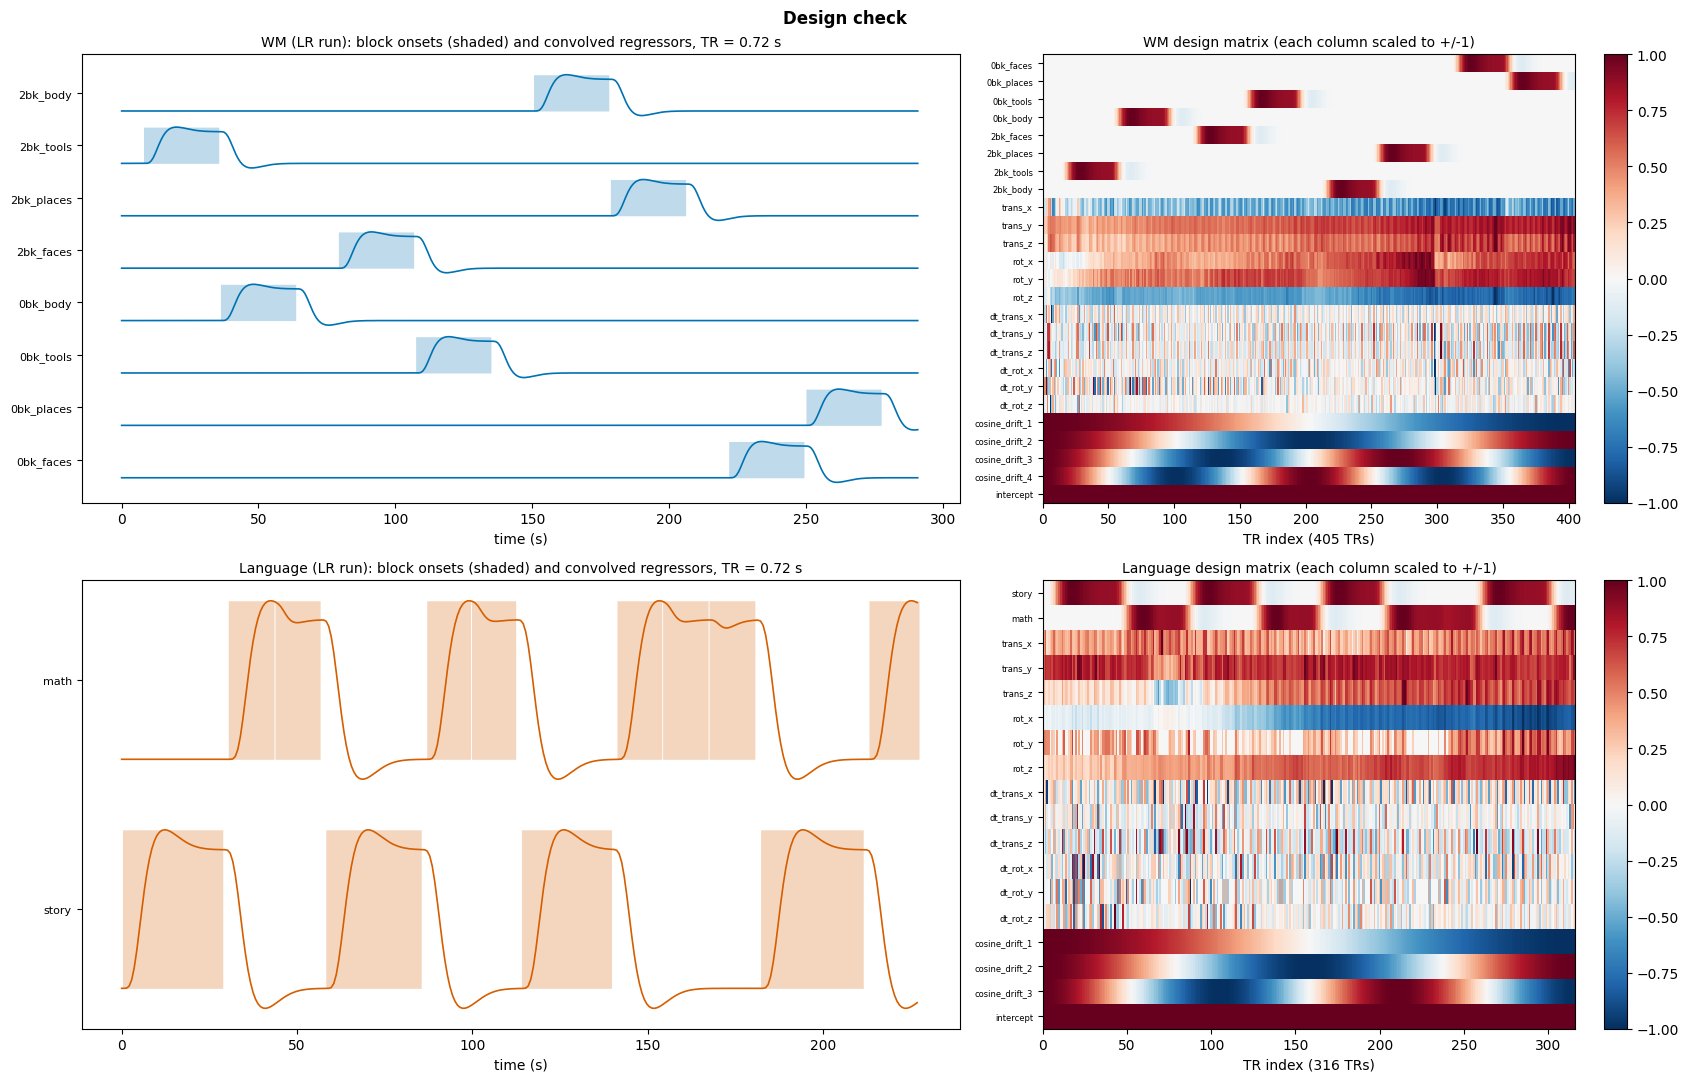
\includegraphics[width=\textwidth]{glm_firstlevel_1}
\caption{Design check for one participant (103414), both tasks, LR run. \textbf{Left:} block onsets (shaded) with the HRF-convolved regressor for each condition; the WM run contains one block per condition, the Language run four Story and four Math blocks. \textbf{Right:} the full design matrix, each column scaled to $\pm1$ --- condition regressors, 12 motion regressors, the discrete cosine drift basis for the 128\,s high-pass filter, and the intercept. The time axis is built from $\mathrm{TR}=0.72$\,s and the frame count read from the file, not from the (incorrect) CIFTI header. Figure produced by Stage~1 of the analysis notebook.}
\label{fig:design}
\end{figure*}

Fig.~\ref{fig:design} shows the resulting design for one participant. Serial correlation was handled by prewhitening \cite{woolrich2001}. We first fitted ordinary least squares, estimated the lag-1 autocorrelation $\rho$ of the residuals at each grayordinate, and binned $\rho$ in steps of 0.005. For each bin we built one whitening matrix from the AR(1) form, whitened the data and design, and refitted by least squares. This gives one fit per bin rather than one per grayordinate, at negligible loss of precision. The outputs are the $\beta$ estimates and $t$-values for each condition against the implicit baseline. The two runs were never merged in the cross-run analyses (LR is used for one half, RL for the other); for the exploratory first-level maps they were combined by inverse-variance fixed effects. Fig.~\ref{fig:runagree} quantifies how much the two runs agree at the first level, and is the reason every reliability measure below is computed across runs rather than within one: at a conventional threshold, fewer than a third of suprathreshold grayordinates reproduce, so a single-run map is not a stable object to build a representational analysis on.

\begin{figure}[t]
\centering
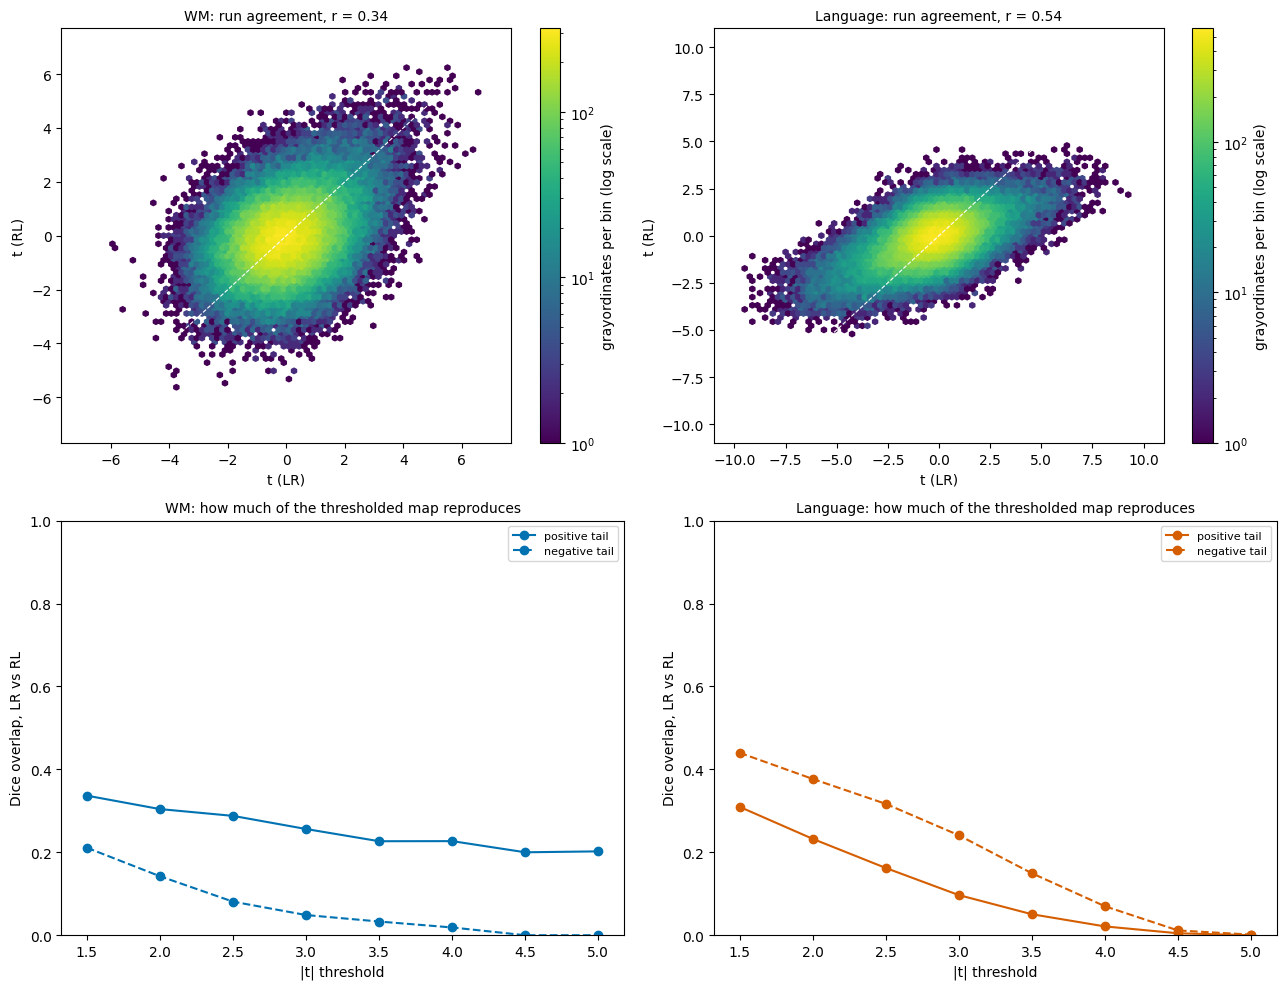
\includegraphics[width=\columnwidth]{glm_firstlevel_4}
\caption{Agreement between the two phase-encoding runs for one participant. \textbf{Top:} the $t$-value of every grayordinate in LR against RL for the WM (left) and Language (right) contrasts, as a log-scaled density. \textbf{Bottom:} Dice overlap of the thresholded maps as a function of the $|t|$ threshold, separately for the positive and negative tails. Overlap falls as the threshold rises, which is expected and is why cross-run validation, not within-run significance, carries the argument in Sections~\ref{sec:rsa}--\ref{sec:decoding}. Figure produced by Stage~1 of the notebook.}
\label{fig:runagree}
\end{figure}

\subsection{Regions of interest}
Eight bilateral ROIs were assembled from Glasser multimodal parcels \cite{glasser2016} (grayordinate counts in brackets): early visual cortex (EVC; V1--V3; 3{,}632), ventral occipito-temporal (OT\textsubscript{ventral}; FFC, VVC, PIT, V8, VMV1--3, PHA1--3; 1{,}850), lateral occipito-temporal (OT\textsubscript{lateral}; LO1--3, V4t, PH; 788), early auditory (A1, LBelt, MBelt, PBelt, RI; 1{,}187), auditory association (A4, A5, STSdp, STSda, STSvp, STSva, STGa, TA2; 2{,}274), dorsolateral frontoparietal (FP\textsubscript{dlpfc}; 46, p9-46v, a9-46v, 9-46d, 8C, 8Av, 8Ad, FEF, IFJp; 3{,}318), parietal (FP\textsubscript{parietal}; IP1, IP2, IP0, IPS1, LIPd, LIPv, VIP, MIP, 7PL; 2{,}460) and cingulate/pre-SMA (SCEF, 6ma, 24dd, p32pr; 1{,}547). ROI definitions are fixed before any decoding and are the same for all participants. Sizes differ by a factor of about four, so accuracy is compared across ROIs with this in mind, and ROI-specific nulls are used rather than a common chance level. Because every later result is conditional on the masks landing where we think they do, Fig.~\ref{fig:roicontrol} reports the positive control: the mean $t$ of each region for each WM condition. Visual regions respond strongly to the pictures and auditory regions do not, which is the pattern the masks must show before any pattern analysis computed in them can be interpreted.

\begin{figure}[t]
\centering
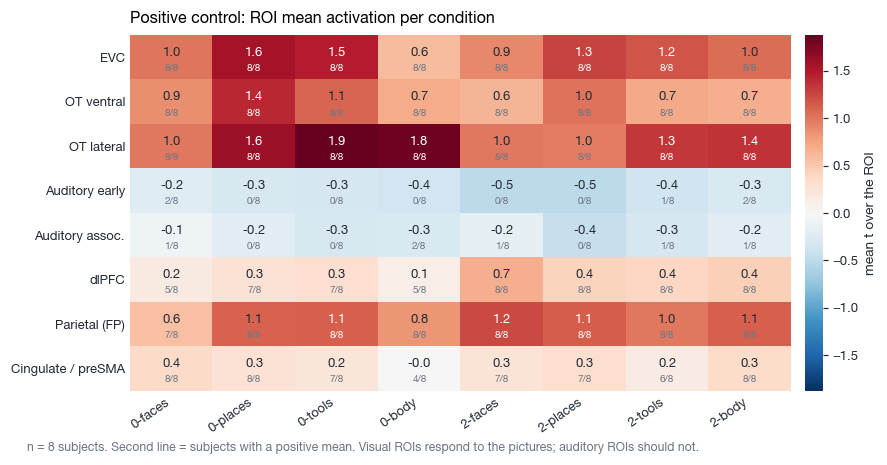
\includegraphics[width=\columnwidth]{roi_mean_activation_positive_control}
\caption{Positive control on the region masks. Each cell is the group-mean $t$ over the region for one WM condition (\Nsub{} participants); the small second number is how many participants had a positive mean. Red indicates activation above the implicit baseline and blue below it. The three visual regions respond positively to all eight picture conditions in every participant (8/8); the two auditory regions are slightly negative throughout, as expected for a silent visual task; and the frontoparietal regions are positive and somewhat stronger under 2-back than 0-back, which is the mean-activation counterpart of the load decoding reported later. Figure produced by Stage~4b of the notebook.}
\label{fig:roicontrol}
\end{figure}

\subsection{Split-half representational similarity}
\label{sec:rsa}
For each participant and ROI, the $t$-maps of the eight WM conditions from LR and RL form two pattern matrices $A,B\in\mathbb{R}^{8\times V}$. Grayordinates with zero variance in either run were dropped.

\textbf{Reproducibility.} Cross-run \emph{identification}: for each condition the LR pattern is correlated with every RL pattern, and the condition is identified correctly when its own RL pattern correlates highest. Chance is $1/8$ for the full set, and 0.5 for pairwise correlation-based identification. This is a within-subject test that needs no classifier.

\textbf{Cross-validated distances.} Distances between conditions $i,j$ are the cross-validated (crossnobis-style) estimate \cite{walther2016,nili2014}
\begin{equation}
d_{ij}=\tfrac{1}{V}\,(\mathbf{a}_i-\mathbf{a}_j)^{\!\top}(\mathbf{b}_i-\mathbf{b}_j),
\end{equation}
symmetrised over the two run assignments. Noise in the two runs is independent, so $\mathbb{E}[d_{ij}]=0$ when two conditions have the same underlying pattern, and negative values are retained. Spatial whitening is not applied (the pre-whitened $t$-maps are used), which we note as a limitation. The $8\times8$ matrix is split into the 0-back block, the 2-back block and the cross-load block. The implementation passes unit tests for symmetry, a zero diagonal, positive mean distance for simulated signal and near-zero mean for noise.

\textbf{Distributed code (voxel removal).} Following Haxby \emph{et al.}\ \cite{haxby2001}, grayordinates were ranked by a one-way $F$ statistic across the four categories, computed in one run only. The top $k\%$ were removed in the \emph{other} run, and identification was recomputed from the remainder. Because removing any grayordinates lowers accuracy, the \emph{excess} loss was compared with removing the same number of randomly selected grayordinates (several random draws). A category code that survives removal of its most selective units, and loses no more than random removal would, is described as distributed.

\textbf{Language reliability.} Because Language has only two conditions, no RDM is possible; we report the cross-run (LR versus RL) correlation of the Math\,$-$\,Story contrast pattern, and use it as the reliability of the Language pattern in the demand analysis of Section~\ref{sec:demand}.

\subsection{Leave-one-subject-out decoding}
\label{sec:decoding}
Decoding was done leave-one-subject-out (LOSO): a classifier is trained on all other participants and tested on the held-out participant, so generalisation is across brains rather than across runs. Features are the ROI pattern of one block (a $t$-map from a single block) with the participant-wise mean across features not removed unless stated. Targets are category (four classes, chance 0.25), load (two classes, chance 0.5), and Math versus Story (chance 0.5).

\textbf{Classifier.} A ridge classifier in dual form with $\lambda=\lambda_{\mathrm{rel}}\,\mathrm{tr}(K)/n$, $\lambda_{\mathrm{rel}}=1$, where $K=XX^{\top}$ is the training Gram matrix; the dual form is used because $V\gg n$. Multi-class problems use one-versus-rest coding. Feature scaling is fitted on the training participants only (fold-local) and applied to the test participant. A linear SVM (\texttt{LinearSVC}, $C=1$, standardised features, fold-local scaling) was run as a cross-check on the same folds to show that conclusions do not rest on the ridge form.

\textbf{Cross-load decoding.} To ask whether the category code is load-invariant at the decoder level, training used one load and testing the other, in both directions, and the result was compared with within-load accuracy.

\textbf{Permutation null.} Labels were permuted $N_{\mathrm{perm}}=1000$ times \emph{within block structure} (category labels shuffled among blocks of the same load and run, load labels among blocks of the same category), so that the null preserves the number of blocks per cell and the run structure. Each permutation reruns the complete LOSO procedure. $p=(1+\#\{\text{null}\ge\text{obs}\})/(N_{\mathrm{perm}}+1)$. Group accuracy is the mean over held-out participants. Bootstrap confidence intervals (10{,}000 resamples) resample \emph{participants}, never blocks.

\subsection{Pattern versus amplitude}
\label{sec:amp}
A multivoxel decoder can exploit differences in the \emph{ROI mean} (an amplitude effect) rather than differences in the spatial pattern \cite{coutanche2013}. Each decoding was therefore repeated after subtracting, within each ROI and block, the mean across grayordinates (and, in a second variant, also dividing by the standard deviation across grayordinates). We also decoded from the ROI mean alone, one feature per block. A region is described as carrying \emph{pattern} information when accuracy survives mean removal, and as \emph{amplitude-driven} when mean-only decoding matches full decoding and pattern-only is at chance. The difference between full and mean-removed accuracy is reported with its participant-level interval. Fig.~\ref{fig:amp} shows this decomposition for load decoding, where it matters most: the two panels separate what the decoder can do from what the region's overall activation does.

\begin{figure*}[t]
\centering
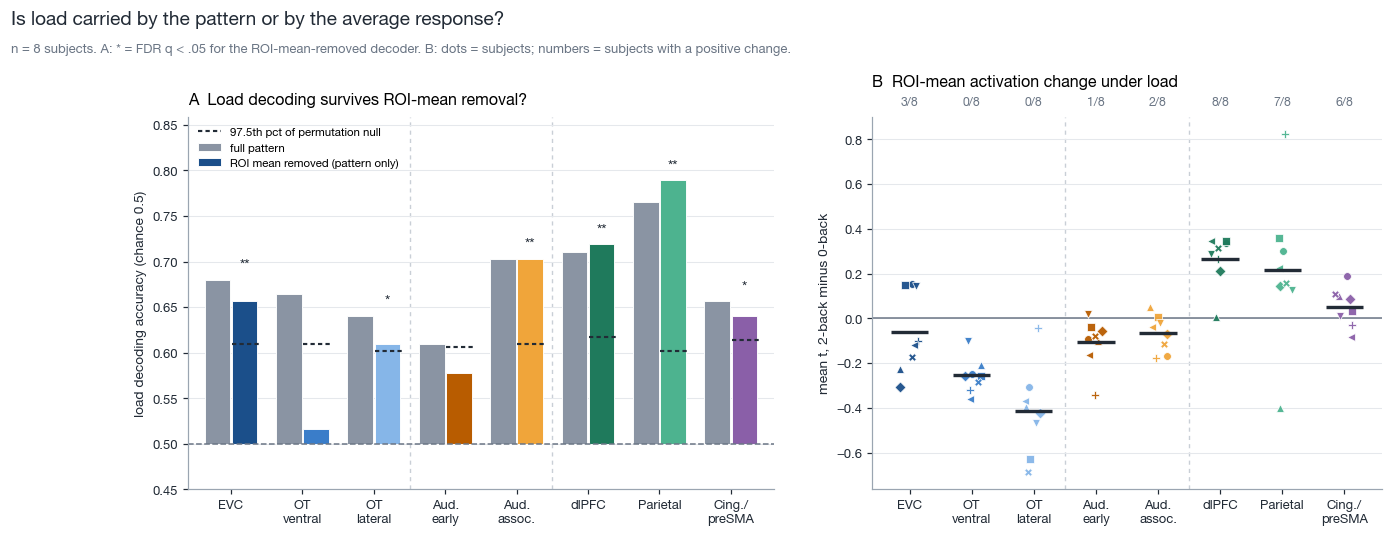
\includegraphics[width=\textwidth]{load_amplitude_vs_pattern}
\caption{Pattern versus amplitude for load decoding (\Nsub{} participants). \textbf{A:} leave-one-subject-out accuracy with the full pattern (grey) and after each block's mean across the region's grayordinates is removed (colour), against the 97.5th percentile of the label-permutation null (dashed). Accuracy that survives mean removal is multivoxel information; accuracy that disappears was an amplitude effect. \textbf{B:} the ROI-mean activation change itself (2-back minus 0-back), one dot per participant, with the number of participants showing a positive change. Note that the two panels can disagree in sign --- a region can carry load in its pattern while its mean response falls --- which is why both are reported. Figure produced by Stage~5e of the notebook.}
\label{fig:amp}
\end{figure*}

\subsection{Load invariance of the category code (H1/H2 model)}
\label{sec:h1}
This is the analysis that operationalises \eqref{eq:rep} on the $8\times8$ cross-run RDM $D$ with entries $d_{(c,l),(c',l')}$ (categories $c,c'$, loads $l,l'$). For each participant and ROI we compute three scalars.

\emph{Within-load distinctness} $\bar d_l$ is the mean of the six off-diagonal category distances within load $l$. \emph{Transfer} is the mean of the cross-load, cross-category distances (e.g.\ face at 0-back versus place at 2-back) minus the mean cross-load, same-category distances (face at 0-back versus face at 2-back); it is positive when categories remain distinguishable across load, i.e.\ when the same code $\mathbf{s}_c$ operates at both loads, and zero when the code is not shared. This numerator is divided by the mean within-load distinctness, $(\bar d_0+\bar d_2)/2$ (\emph{normalised transfer}: 1 means the same code at both loads, 0 means none). Dividing each participant's numerator by that participant's own denominator is unstable when the denominator is near zero, so in the group analysis every participant's numerator is divided by the \emph{group-mean} within-load distinctness instead. \emph{Gain} is $\bar d_2/\bar d_0$: in the model $d\propto g_l^2$, so a ratio below 1 means that load weakens the code. Gain is formed per participant and is undefined (flagged, not silently dropped) where $\bar d_0\le0$; it is unstable when $\bar d_0$ is near zero.

\begin{figure*}[t]
\centering
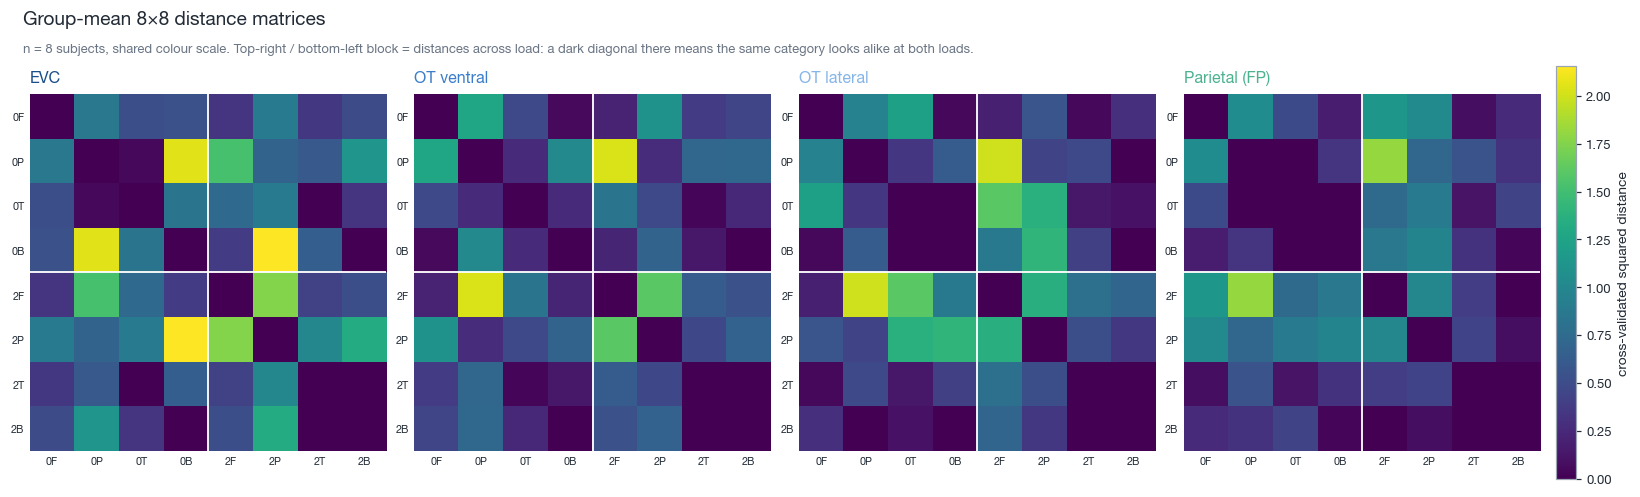
\includegraphics[width=\textwidth]{h1_group_rdms}
\caption{The object the H1 statistics are computed from: group-mean $8\times8$ cross-validated distance matrices (\Nsub{} participants, shared colour scale), shown for the regions that pass the interpretability gate. Rows and columns are load (0 or 2) crossed with category (F faces, P places, T tools, B body). The two diagonal blocks are the within-load category distances that give $\bar d_0$ and $\bar d_2$; the off-diagonal blocks are the cross-load distances from which transfer is computed as (different-category $-$ same-category). The load main effect is present in both terms of that difference and cancels, so what the transfer term measures is the category information that survives the change of load. Figure produced by Stage~9a of the notebook.}
\label{fig:grouprdm}
\end{figure*}

Fig.~\ref{fig:grouprdm} shows the matrices these three scalars summarise.

\textbf{Interpretability gate.} A transfer or gain is interpreted only when within-load distinctness is reliably above zero in that ROI (sign-flip test across participants, FDR-corrected), because the ratios are not meaningful where there is no category information to preserve. The original statistic of Section~\ref{sec:failed}, the Spearman correlation $\rho$ between the two six-pair sub-RDMs, is still computed for comparison only.

\textbf{What transfer does and does not assert.} A transfer or retention near 1 means that the \emph{category} dimension of the representation is preserved across load. It does not mean that load has no effect: load itself is decodable in every region examined, and the representation can move along a separate load axis while the category axis is unchanged. Equally, because these are block-level estimates spanning stimulus presentation and response, nothing in them distinguishes a stimulus-driven code from one maintained over a delay. Cross-load generalisation is sufficient but not necessary evidence of a shared code --- a code that is shared but rotated would be missed by a linear decoder, which is one reason the geometry measure is reported alongside the decoding measure. Finally, a transfer value computed in a region without measurable category geometry is uninterpretable whatever its size, which is what the interpretability gate below enforces.

\textbf{Null.} Condition labels cannot be shuffled freely because the design has structure. We permuted the pairing between categories at 2-back and categories at 0-back (all $4!=24$ relabelings, of which one is the identity) and recomputed transfer; the observed value is ranked within these 24. Since the smallest p-value is 1/24, we treat this as a descriptive reference rather than the primary test, and carry the inference by the participant-level tests below.

\textbf{Equivalence (TOST).} Failing to reject a difference is not evidence of equality. For the claim of invariance we ran two one-sided tests \cite{schuirmann1987} across participants, with equivalence margins fixed before looking at the results: $\pm0.25$ for pooled-normalised transfer and $\pm0.10$ for the decoding-accuracy loss across load. Invariance is claimed only when both one-sided p-values are below $0.05$ (after FDR), and we additionally report the smallest margin $m_{\min}$ at which equivalence would hold, so that the reader can judge the result against a stricter or looser margin.

\subsection{Matched resting-state null}
\label{sec:rest}
A pipeline can produce non-zero decoding, transfer or gain even on data with no task, because of the temporal and spatial structure of the signal. To obtain a null with the \emph{same} structure, we drew random windows of 405 consecutive frames from the participant's cleaned resting-state runs, imposed the participant's real WM design on each window, and ran the identical pipeline (GLM, RDM, H1 statistics). Repeating this gives a null distribution for every statistic in Sections~\ref{sec:rsa}--\ref{sec:h1}; the observed statistic is compared with the empirical distribution (one-sided, $p=(1+\#\ge)/(n+1)$) and with the participant-level mean. Resting data are currently available for one participant, so the null is reported for that participant and is not yet used for group inference. Fig.~\ref{fig:restnull} shows the form this null takes for the primary transfer statistic.

\begin{figure*}[t]
\centering
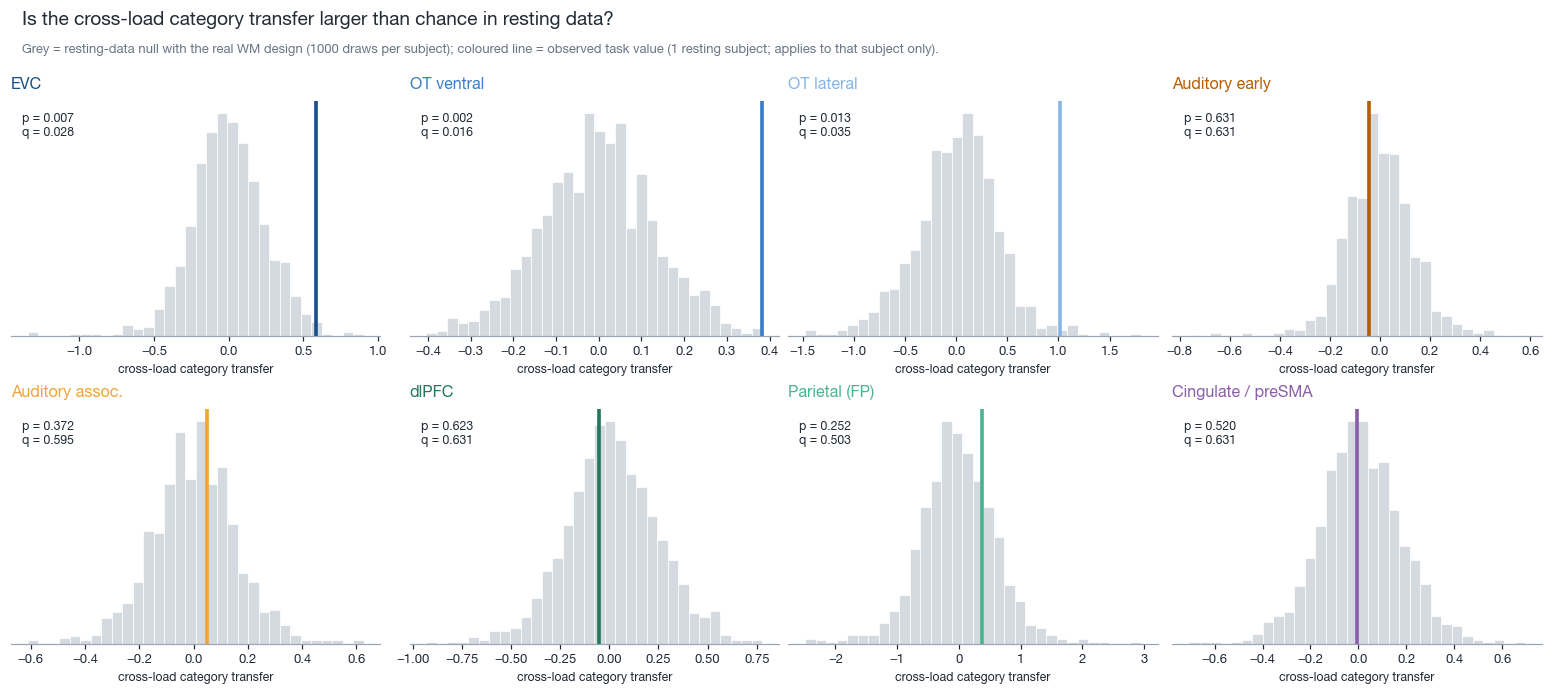
\includegraphics[width=\textwidth]{rfmri_null_transfer}
\caption{The matched resting-state null for the cross-load category transfer, one panel per region. Grey histograms are the values the complete pipeline returns on 1{,}000 random 405-frame windows of resting-state data with the real WM design imposed on them; the coloured line is the observed task value, and the inset gives the empirical $p$ and its FDR-corrected $q$. Because the windows contain no task, the grey distribution is what the design, the AR(1) GLM and the noise structure produce on their own, which is the only fair reference for a statistic of this kind. Figure produced by Stage~6a of the notebook; currently one participant has resting runs, so these $p$-values apply to that participant alone.}
\label{fig:restnull}
\end{figure*}

\subsection{Cross-task decoding and the shared demand axis}
\label{sec:demand}
\textbf{Cross-task decoder.} H4 asks whether a pattern that separates 2-back from 0-back in the visual WM task also separates Math from Story in the auditory Language task. In direction A a ridge classifier is trained on WM load (0-back versus 2-back) in the other participants and applied to the held-out participant's Language blocks; in direction B it is trained on Language (Story versus Math) and tested on WM load. The mapping Math $\leftrightarrow$ 2-back is fixed before the analysis (Math is the more demanding condition); accuracy below 0.5 would mean that the mapping is reversed. The analysis was repeated for the full pattern, the ROI-mean-removed pattern and the ROI mean alone, and each is judged separately, so that a result that transfers only through the mean is not reported as shared pattern information.

\textbf{Inference.} The participant is the unit. Each participant's accuracy $a$ is treated as exchangeable with $1-a$ under the null, and the group mean is compared with the $2^n$ sign-flipped means (exact for $n\le14$). The smallest attainable two-sided $p$ is $2/2^n$, i.e.\ $0.0078$ at $n=8$. P-values are corrected by Benjamini--Hochberg FDR \cite{benjamini1995} across ROIs and directions. We also report the number of participants above 0.5, since a mean driven by two participants is not a group effect.

\textbf{Demand-axis correlation.} For each ROI we form the demand pattern (2-back minus 0-back, averaged over categories) and the Language pattern (Math minus Story) from independent runs, and correlate them across grayordinates between different runs (LR of one task with RL of the other and vice versa, averaged), which removes the shared-noise correlation within one run. The correlation is compared with the within-task cross-run correlations of each pattern, and a reliability-corrected value (dividing by the geometric mean of the two within-task LR/RL reliabilities, an attenuation correction) is reported only where both reliabilities exceed 0.2, because the correction diverges for near-zero reliabilities. Participant-level significance uses the sign-flip test.

\textbf{Mantel test and noise ceiling.} To compare the representational structure of the $4\times4$ category RDMs between the two loads we use a Mantel test (5{,}000 joint permutations of the category labels on both axes of one RDM) with Spearman and Kendall rank correlations \cite{mantel1967}; confidence intervals resample participants. A descriptive noise ceiling is obtained, per ROI and load, by correlating each participant's RDM with the mean RDM of the others (lower bound) and with the mean including the participant (upper bound); it is reported only with at least three participants.

\subsection{Confirmatory checks on Story versus Math}
\label{sec:langcheck}
Story-versus-Math decoding reaches or approaches ceiling in nearly every region, including visual ones, and that result needs to be qualified rather than quoted. Two properties of the design make a high accuracy cheap. First, each run contributes exactly two blocks, so after the within-run mean is removed the Story and Math patterns are exact mirror images: a participant contributes one direction in pattern space per run, and the classifier only has to recover the sign of a single group-mean difference pattern. A difference that is very small but consistent in direction across participants therefore decodes perfectly. Second, Story and Math differ in difficulty, block length and motor output as well as in linguistic content, so a brain-wide shift between the two conditions is plausible, and a brain-wide shift reaches every region.

We therefore repeat the analysis in four versions --- the full pattern; the pattern with each block's ROI mean removed; the ROI mean alone; and the pattern after subtracting the mean over the union of all eight ROIs, as a proxy for a global shift --- under two cross-validation schemes, the second of which trains on one phase-encoding run of the other participants and tests the other run of the held-out participant, so that training and test data never come from the same acquisition. Inference uses the exact participant-level sign-flip test of Section~\ref{sec:demand} rather than the block-label permutation, for the same reason as there: with two mirror-image samples per run the block-level null is far too narrow. We also report the within-participant cross-run reliability of the Math\,$-$\,Story pattern, because a region can be decoded at ceiling across participants while its own pattern barely reproduces between two runs of the same brain --- the signature of a weak but highly consistent difference. A visual region is described as carrying Story/Math \emph{pattern} information only if the mean-removed decoder works \emph{and} accuracy survives global-signal removal.

\subsection{Controls on the parietal category code}
\label{sec:parietal}
The parietal region is the only non-visual region in which stimulus category is decodable, and it also shows the smallest loss of category information across load, so it carries most of the novelty of the analysis and attracts most of the scepticism. Four alternative accounts are therefore tested one at a time before the result is described as an abstract category code. (i) \emph{One dominant contrast:} all six category pairs are decoded separately, since a four-way decoder can exceed chance while separating only faces from places. (ii) \emph{Activation ranking:} the four-way decoding is repeated with each block's ROI mean removed and from the ROI mean alone, as in Section~\ref{sec:amp}. (iii) \emph{Spillover from visual cortex:} intraparietal parcels border V3A/V7, so grayordinates are split at the median of their mean response across all eight WM conditions and category decoding is run separately in the more and the less visually driven half; the split uses the mean over categories, which the category preprocessing removes, so the selection carries no information about the labels. (iv) \emph{Region size:} every region is subsampled to the same number of grayordinates over several random draws, which also makes explicit that the dorsolateral prefrontal region has more grayordinates and no category code. Finally, the group category RDM of the parietal region is compared with that of ventral occipito-temporal cortex by a Mantel test, since a code inherited from vision would share its geometry whereas an independent code would not. None of these re-tests the existence of the code, which Section~\ref{sec:decoding} establishes by permutation; they determine how it may be described.

\subsection{Event-timing audit}
\label{sec:timing}
Cross-participant decoding can be inflated when the stimulus schedule is shared across participants, because anything locked to the schedule (scanner drift, respiratory or cardiac phase, low-frequency fluctuations common to the group) then becomes a predictor of the label. For every participant and run we extracted block onsets and compared them across participants, calling two schedules ``shared'' when all onsets agree within 0.5\,s. For each task we report the number of distinct schedules, the largest onset difference, and a verdict. Where schedules are shared, a leave-one-category-out check and the ROI-mean-removed analysis of Section~\ref{sec:amp} are used to judge whether an effect depends on the schedule. Fig.~\ref{fig:timing} shows the schedule itself for the reference participant. In our data the WM schedule is shared within about 0.32\,s across participants, while the Language schedule differs between participants; consequently, label effects that are specific to one category and a fixed position in the schedule (places, in particular) are interpreted cautiously.

\begin{figure*}[t]
\centering
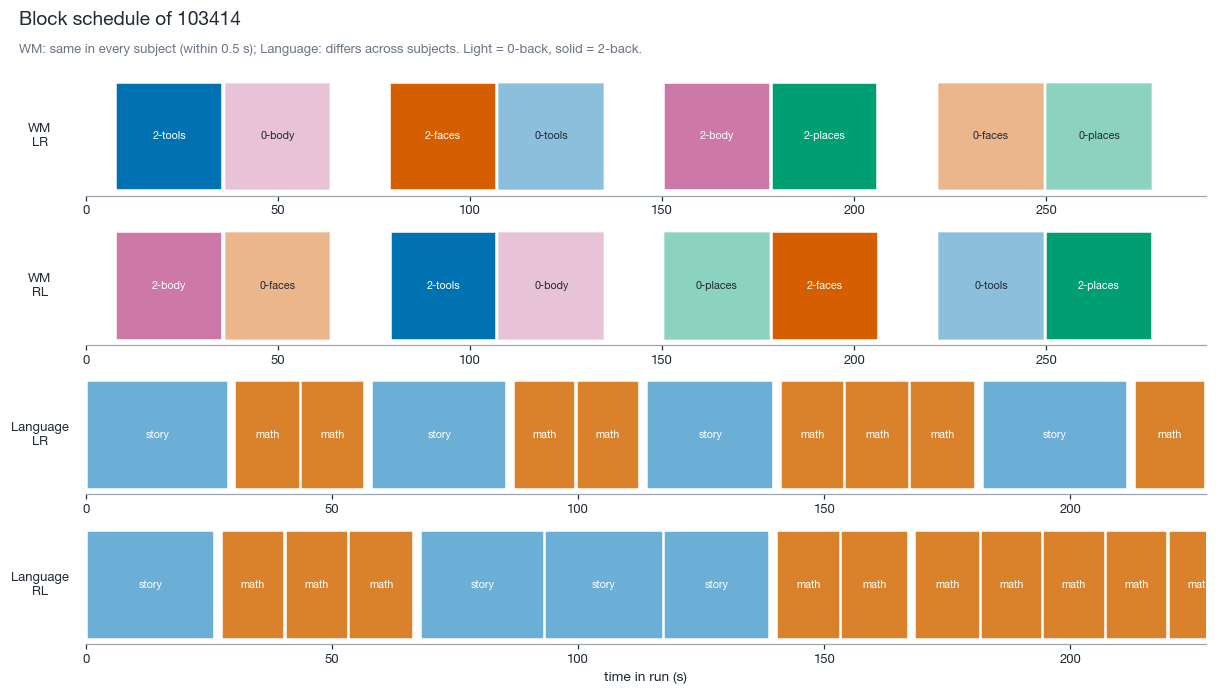
\includegraphics[width=\textwidth]{event_timing_schedule}
\caption{Block schedule of the reference participant for both tasks and both runs, reconstructed from the HCP EV files. Colour denotes category (or Story/Math); light blocks are 0-back and solid blocks 2-back. The WM schedule is identical across participants to within 0.32\,s, so any signal locked to this timeline --- drift, slow physiological fluctuation, or simply position in the run --- is shared by every participant and can be read out by a cross-participant decoder as if it were a category or load code. The figure makes the specific risk visible: ``places'' blocks sit late in both WM runs. The Language schedule differs across participants, so no shared timing artefact can produce the Language effects. Figure produced by Stage~11 of the notebook.}
\label{fig:timing}
\end{figure*}

\subsection{Statistical inference}
Throughout, the participant is the unit of replication. Group statistics are either exact sign-flip tests (for statistics that are symmetric around a null value), label-permutation tests that re-run the complete pipeline, or participant bootstrap intervals; none treats blocks or grayordinates as independent. Multiple comparisons are controlled by Benjamini--Hochberg FDR \cite{benjamini1995} within families that are fixed before the analysis (the confirmatory family is the set of ROI $\times$ target tests for H1--H4; anything else is exploratory and labelled so). With $n=8$ the exact sign-flip test has a smallest p-value of $0.0078$ (two-sided), so the results are interpreted through effect sizes and intervals as much as p-values, and a result that rests on the smallest attainable p-value is flagged.

\subsection{Approaches tried and abandoned}
\label{sec:failed}
Two analyses that we implemented did not hold up and were replaced; we report them to explain choices made above.

\textbf{(1) A six-pair rank-correlation statistic for invariance.} The first version of H1 compared the 0-back and 2-back category RDMs by a single Spearman correlation over their $\binom{4}{2}=6$ off-diagonal entries, as is common in the RSA literature \cite{kriegeskorte2008,nili2014}. With six pairs the statistic takes few distinct values and is dominated by ties and a single misordered pair, so it is highly variable even under the null: in the one resting-state participant processed with the matched null of Section~\ref{sec:rest}, the null distribution of $\rho$ was very wide (standard deviation about 0.46), and the BH-adjusted $q$ for that participant was $\approx0.996$, i.e.\ the statistic could not separate signal from the null. It also cannot express equivalence: a non-significant correlation is not evidence of a shared code, and a high one does not rule out a change of scale. We replaced it by the full $8\times8$ model with separate transfer and gain terms, the permutation reference, and the TOST of Section~\ref{sec:h1}. The Mantel/Spearman comparison of Section~\ref{sec:demand} is kept only as a descriptive companion.

\textbf{(2) A block-level label-flip null for cross-task decoding.} We first assessed cross-task decoding by permuting (flipping) the labels of individual test blocks. The Story-versus-Math pattern is nearly identical across participants, and the test blocks of one participant (and of different participants, where the schedule is shared) are not independent samples, so the null was far too narrow and returned $p$-values that were too small even for effects we could not otherwise support, an anti-conservative test. We replaced it by the participant-level exact sign-flip test of Section~\ref{sec:demand}, accepting that its smallest p is $2/2^n$. A related bug found at the same stage, in which a verdict rule declared ``no transfer'' whenever the full-pattern accuracy was below 0.6 even though the pattern-only decoder transferred, was fixed by judging the pattern-only and mean-only decoders separately.

\subsection{Limitations of the methods}
Two checks are not yet done: a spatial (spin) permutation test that would keep the cortical autocorrelation when relating ROI maps (it needs the sphere files), and the resting-state null for all participants. With $n=\Nsub$ the analyses are best read as a pilot, and no formal power calculation was performed. The ROI definitions come from a group-based parcellation, and the largest ROIs contain about four times as many grayordinates as the smallest, so ROI comparisons are descriptive.

\section{Results}
\emph{To be completed.}

\section{Discussion and Conclusion}
\emph{To be completed.}

\begin{thebibliography}{00}
\bibitem{vanessen2013} D. C. Van Essen \emph{et al.}, ``The WU-Minn Human Connectome Project: an overview,'' NeuroImage, vol. 80, pp. 62--79, 2013.
\bibitem{barch2013} D. M. Barch \emph{et al.}, ``Function in the human connectome: task-fMRI and individual differences in behavior,'' NeuroImage, vol. 80, pp. 169--189, 2013.
\bibitem{drobyshevsky2006} A. Drobyshevsky, S. B. Baumann, and W. Schneider, ``A rapid fMRI task battery for mapping of visual, motor, cognitive, and emotional function,'' NeuroImage, vol. 31, pp. 732--744, 2006.
\bibitem{kanwisher1997} N. Kanwisher, J. McDermott, and M. M. Chun, ``The fusiform face area: a module in human extrastriate cortex specialized for face perception,'' J. Neurosci., vol. 17, pp. 4302--4311, 1997.
\bibitem{epstein1998} R. Epstein and N. Kanwisher, ``A cortical representation of the local visual environment,'' Nature, vol. 392, pp. 598--601, 1998.
\bibitem{downing2001} P. E. Downing \emph{et al.}, ``A cortical area selective for visual processing of the human body,'' Science, vol. 293, pp. 2470--2473, 2001.
\bibitem{duncan2010} J. Duncan, ``The multiple-demand (MD) system of the primate brain: mental programs for intelligent behaviour,'' Trends Cogn. Sci., vol. 14, pp. 172--179, 2010.
\bibitem{haxby2001} J. V. Haxby \emph{et al.}, ``Distributed and overlapping representations of faces and objects in ventral temporal cortex,'' Science, vol. 293, pp. 2425--2430, 2001.
\bibitem{kriegeskorte2008} N. Kriegeskorte, M. Mur, and P. Bandettini, ``Representational similarity analysis --- connecting the branches of systems neuroscience,'' Front. Syst. Neurosci., vol. 2, art. 4, 2008.
\bibitem{emrich2013} S. M. Emrich, A. C. Riggall, J. J. LaRocque, and B. R. Postle, ``Distributed patterns of activity in sensory cortex reflect the precision of multiple items maintained in visual short-term memory,'' J. Neurosci., vol. 33, pp. 6516--6523, 2013.
\bibitem{kriegeskorte2013} N. Kriegeskorte and R. A. Kievit, ``Representational geometry: integrating cognition, computation, and the brain,'' Trends Cogn. Sci., vol. 17, pp. 401--412, 2013.
\bibitem{bernardi2020} S. Bernardi \emph{et al.}, ``The geometry of abstraction in the hippocampus and prefrontal cortex,'' Cell, vol. 183, pp. 954--967, 2020.
\bibitem{binder2011} J. R. Binder \emph{et al.}, ``Mapping anterior temporal lobe language areas with fMRI: a multicenter normative study,'' NeuroImage, vol. 54, pp. 1465--1475, 2011.
\bibitem{woolrich2001} M. W. Woolrich, B. D. Ripley, M. Brady, and S. M. Smith, ``Temporal autocorrelation in univariate linear modeling of fMRI data,'' NeuroImage, vol. 14, pp. 1370--1386, 2001.
\bibitem{walther2016} A. Walther \emph{et al.}, ``Reliability of dissimilarity measures for multi-voxel pattern analysis,'' NeuroImage, vol. 137, pp. 188--200, 2016.
\bibitem{nili2014} H. Nili \emph{et al.}, ``A toolbox for representational similarity analysis,'' PLoS Comput. Biol., vol. 10, e1003553, 2014.
\bibitem{coutanche2013} M. N. Coutanche, ``Distinguishing multi-voxel patterns and mean activation: why, how, and what does it tell us?,'' Cogn. Affect. Behav. Neurosci., vol. 13, pp. 667--673, 2013.
\bibitem{haynes2006} J.-D. Haynes and G. Rees, ``Decoding mental states from brain activity in humans,'' Nat. Rev. Neurosci., vol. 7, pp. 523--534, 2006.
\bibitem{stelzer2013} J. Stelzer, Y. Chen, and R. Turner, ``Statistical inference and multiple testing correction in classification-based multi-voxel pattern analysis (MVPA),'' NeuroImage, vol. 65, pp. 69--82, 2013.
\bibitem{nichols2002} T. E. Nichols and A. P. Holmes, ``Nonparametric permutation tests for functional neuroimaging: a primer with examples,'' Hum. Brain Mapp., vol. 15, pp. 1--25, 2002.
\bibitem{glasser2016} M. F. Glasser \emph{et al.}, ``A multi-modal parcellation of human cerebral cortex,'' Nature, vol. 536, pp. 171--178, 2016.
\bibitem{robinson2014} E. C. Robinson \emph{et al.}, ``MSM: a new flexible framework for multimodal surface matching,'' NeuroImage, vol. 100, pp. 414--426, 2014.
\bibitem{salimi2014} G. Salimi-Khorshidi \emph{et al.}, ``Automatic denoising of functional MRI data: combining independent component analysis and hierarchical fusion of classifiers,'' NeuroImage, vol. 90, pp. 449--468, 2014.
\bibitem{benjamini1995} Y. Benjamini and Y. Hochberg, ``Controlling the false discovery rate: a practical and powerful approach to multiple testing,'' J. R. Stat. Soc. B, vol. 57, pp. 289--300, 1995.
\bibitem{schuirmann1987} D. J. Schuirmann, ``A comparison of the two one-sided tests procedure and the power approach for assessing the equivalence of average bioavailability,'' J. Pharmacokinet. Biopharm., vol. 15, pp. 657--680, 1987.
\bibitem{mantel1967} N. Mantel, ``The detection of disease clustering and a generalized regression approach,'' Cancer Res., vol. 27, pp. 209--220, 1967.
\end{thebibliography}

\end{document}
